
  \section{Auswertung}
  \subsection{Bestimmung der maximalen Kraftflussdichte}
  Die gemessenen Werte sind relativ zum Mittelpunkt der Helmholtzspule aufgenommen.
  An diesem Punkt ist das Magnetfeld am größten.
  Die Werte sind in Tabelle \ref{tab:Bfeld} zu finden.

  \begin{table}
    \centering
    \caption{gemessene Kraftflussdichte}
    \label{tab:Bfeld}
    \begin{tabular}{c c}
      \toprule
      B(z)/ \si{\milli\tesla} & $\symup{z_{rel}}$ / \si{\centi\meter}\\
      \midrule
       68  & 14\\
       136 & 12\\
       254 & 10\\
       350 & 8 \\
       407 & 6 \\
       436 & 4 \\
       450 & 2 \\
       464 & 0 \\
       458 & -2\\
       451 & -4\\
       437 & -6\\
       404 & -8\\
       335 &-10\\
       210 &-12\\
       98  &-14\\
      \bottomrule
    \end{tabular}
  \end{table}

Um die maximale Kraftflussdichte zu ermitteln wird B(z) gegen z aufgetragen.
Dies ist in Abbildung \ref{fig:Bfeld} zu sehen.
Die lineare Regression wird mit der Formel
\begin{equation*}
 B(z) = m \cdot (z-a)^2 + n
\end{equation*}
durchgeführt.
So ergeben sich die Parameter
\begin{align*}
m &= (-2,01 \pm 0,08)\,\mathrm{\frac{mT}{cm^2}}\\
a &= (-0,62 \pm 0,16)\,\mathrm{cm}\\
n &= (481,17 \pm 8,13)\,\mathrm{mT}\\
\Rightarrow S &=(-0,62, 481,17)
\end{align*}
Somit liegt das Maximum bei
\begin{equation}
\symup{B_{max}}= (481,17\pm 8,13)\,\mathrm{mT} .
\label{eqn:bfeld}
\end{equation}
\begin{figure}
  \centering
  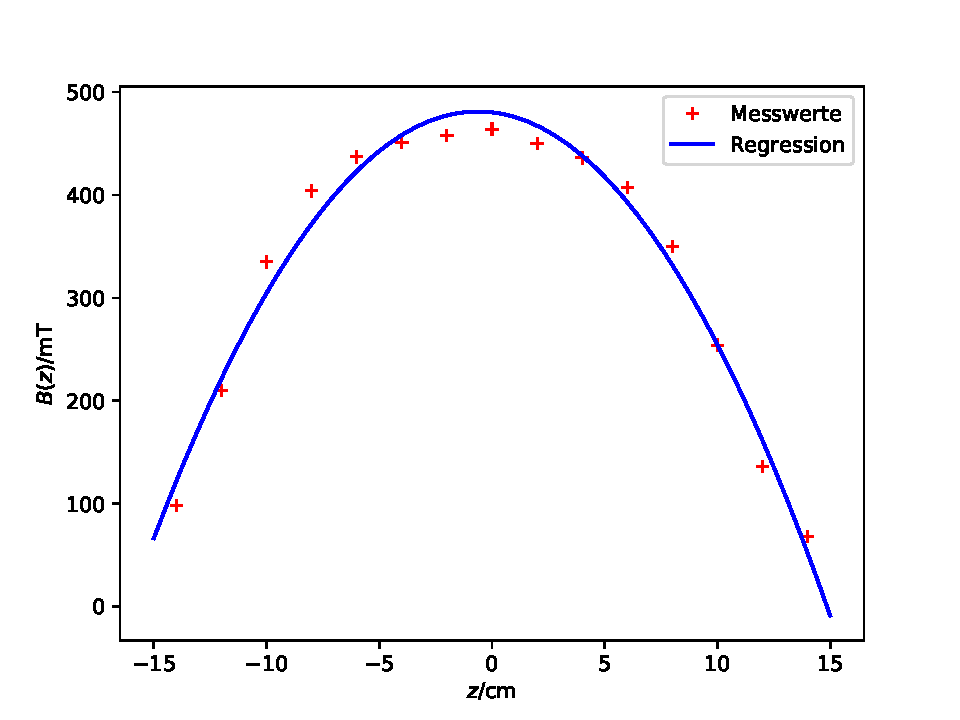
\includegraphics[width=\textwidth]{plotbfeld.pdf}
  \caption{gemessene Kraftflussdichte}
  \label{fig:Bfeld}
\end{figure}

\subsection{Messung der Faraday-Rotation}
Die Messergebnisse des n-dotierten GaAs sind in Tabelle \ref{tab:ndotiert} aufgetragen.
Die Probe hat eine Dicke von D=$1,36\,\mathrm{mm}$ und N=$1,2\cdot 10^{18}\,\mathrm{cm^3}$.

  \begin{table}
    \centering
    \caption{n-dotiertes GaAs}
    \label{tab:ndotiert}
    \begin{tabular}{c c c c c}
      \toprule
      $\lambda/ \si{\micro\meter}$ & $\theta_1 / °$ & $\theta_2 /°$ & $\theta_{\symup{reell}}/°$ &
      $\Delta\theta_{\symup{norm}}/\frac{°}{\mathrm{m}}$\\
      \midrule
       1,06  & 189 & 186 & 1,5 & 1102,94\\
       1,29  & 190 & 188 & 1,0 & 735,29\\
       2,34  & 211 & 210 & 0,5 & 367,64\\
       2,51  & 213 & 210 & 1,5 & 1102,94\\
       2,9   & 306 & 283 & 11,5& 8455,88\\
       3,18  & 223 & 208 & 7,5 & 5514,70\\
       3,985 & 320 & 312 & 4,0 & 2941,18\\
       5,3   & 231 & 216 & 7,5 & 5,51\\
       \bottomrule
    \end{tabular}
  \end{table}

  Die Messergebnisse der hochreinen Probe
  mit einer Dicke von $D=5,1\,\mathrm{mm}$ sind in Tabelle \ref{tab:hochrein} aufgetragen.

  \begin{table}
    \centering
    \caption{hochreines GaAs}
    \label{tab:hochrein}
    \begin{tabular}{c c c c c}
      \toprule
      $\lambda/ \si{\micro\meter}$ & $\theta_1 / °$ & $\theta_2 /°$ & $\theta_{\symup{reell}}/°$ &
      $\Delta\theta_{\symup{norm}}/\frac{°}{\mathrm{m}}$\\
      \midrule
       1,06  & 208 & 207 & 0,5 & 0,10\\
       1,29  & 200 & 198 & 1,0 & 0,20\\
       2,34  & 208 & 206 & 1,0 & 0,20\\
       2,51  & 209 & 207 & 1,0 & 0,20\\
       2,9   & 234 & 228 & 4,0 & 0,59\\
       3,18  & 238 & 220 & 9,0 & 1,76\\
       3,985 & 223 & 215 & 4,0 & 0,78\\
       5,3   & 259 & 250 & 4,5 & 0,88\\
       \bottomrule
    \end{tabular}
  \end{table}

  $\theta_{\symup{reel}}$ entspricht hierbei der halbierten Differenz von $\theta_1$ und $\theta_2$.
  $\theta_{\symup{norm}}$ ist der längennormierte Winkel.
  In Abbildung \ref{fig:b} wurde der längennormierte Winkel gegen das quadrat der Wellenlänge aufgetragen
  \begin{figure}
    \centering
    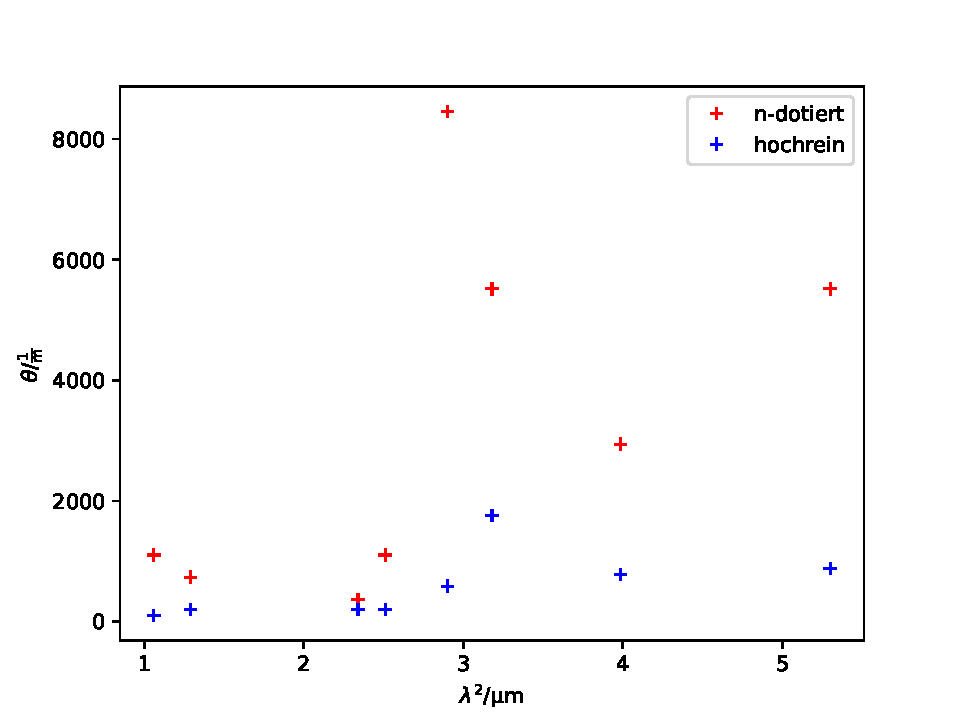
\includegraphics[width=\textwidth]{plotGaAs.pdf}
    \caption{Der Winkel gegen $\lambda ^2$ }
    \label{fig:b}
  \end{figure}

\subsection{Bestimmung der effektiven Masse}
Zur Bestimmung der effektiven Masse wird die Differenz der beiden normierten Winkel der n-dotierten
und der hochreinen Probe gebildet. Die Ergebisse sind in Tabelle \ref{tab:dif} zu finden.
Diese Winkel, aufgetragen gegen die Wellenlänge zum Quadrat, werden in Abbildung \ref{fig:dif} dargestellt.


\begin{table}[H]
  \centering
  \caption{n-dotiertes GaAs}
  \label{tab:dif}
  \begin{tabular}{c c c c c}
    \toprule
    $\lambda/ \si{\micro\meter}$ & $\theta_{\symup{diff}} / \frac{°}{m}$ \\
    \midrule
     1,06  & 1005,09\\
     1,29  & 539,60\\
     2,34  & 171,95\\
     2,51  & 907,25\\
     2,9   & 7868,80\\
     3,18  & 3753,45\\
     3,985 & 2158,40\\
     5,3   & 4634,08\\
     \bottomrule
  \end{tabular}
\end{table}
\begin{figure}[H]
  \centering
  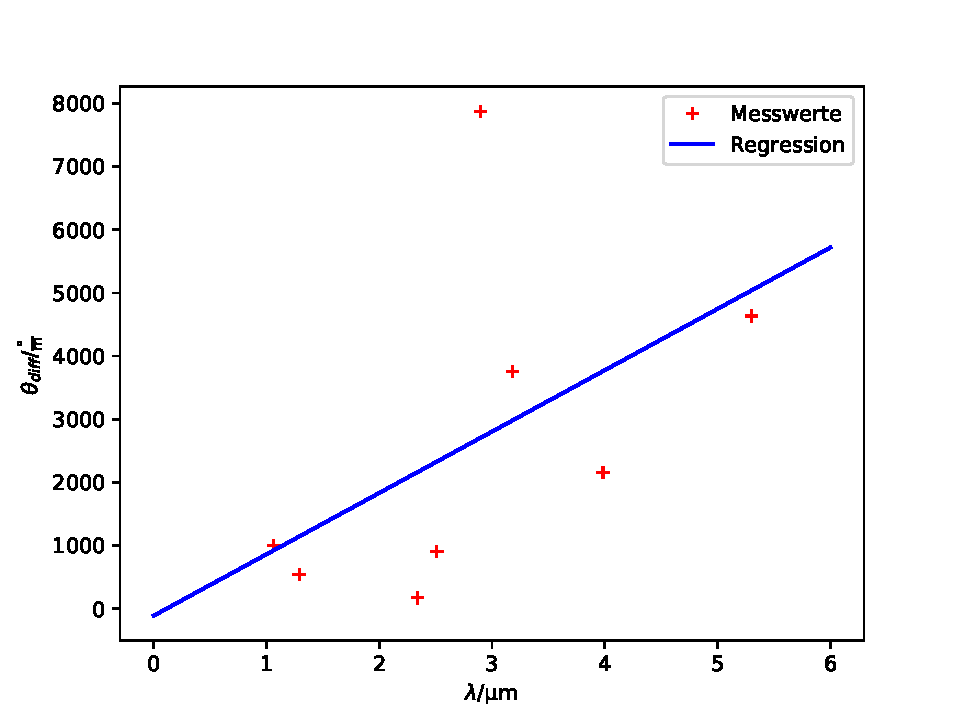
\includegraphics[width=\textwidth]{tdiff.pdf}
  \caption{Die Winkeldifferenz gegen $\lambda ^2$ }
  \label{fig:dif}
\end{figure}
Die linerare Regression wurde mit
\begin{equation*}
  \theta(\lambda^2) = a\cdot \lambda^2 +b
\end{equation*}
durchgeführt.
Die Parameter lauten:
\begin{align*}
  a &= (1,0\pm0,7) \cdot 10^{3}\,\mathrm{\frac{1}{\mu m^3}}\\
  b &= (-0,1\pm2,1)\cdot 10^{3}\,\mathrm{\frac{1}{m}}
\end{align*}

Mit Formel \ref{eqn:meff} ergibt sich
\begin{equation*}
a = \frac{e_0^3}{8\pi^2\epsilon_0c^2}\frac{1}{m*^2}\frac{NB}{n}
\end{equation*}
Dabei ist n der Brechungsindex und liegt bei n=3,6.\cite{Brechungsindex}
Nach der effektiven Masse umgestellt wird die Formel zu
\begin{equation*}
  m* =\sqrt{\frac{e_0^3}{8\pi^2\epsilon_0c^2}\frac{1}{a}\frac{NB}{n}}.
\end{equation*}
Der Wert für B wird aus \ref{eqn:bfeld} übernommen und der für N liegt,
wie oben bereits erwähnt, bei N=$1,2\cdot 10^{18}\,\mathrm{cm^3}$.
Somit lautet das Ergebnis für die effektive Masse:
\begin{equation*}
  m* =(6,0\pm 2,1)\cdot10^{-34}\, \mathrm{kg}
\end{equation*}
Der Fehler berechnet sich mit
\begin{equation*}
  \Delta m* = \sqrt{\left(\frac{dm*}{dB}\cdot \Delta B\right)+\left(\frac{dm*}{da}\cdot \Delta a\right)^2}
\end{equation*}

\section{Diskussion}

Die Messung der Kraftflussdichte hat gut funktioniert.
An der Abbildung \ref{fig:Bfeld} ist zu erkennen, dass die gemessenen Werte nicht stark von der Regression abweichen.
So sind auch die Fehler der Parameter eher gering.

Die Messung der Faraday-Rotation war schwierig, da die Sinuswelle am Oszilloskop stark geflackert und geschwankt hat.
Außerdem wurde bei größeren Wellenlängen weniger Licht vom Interferenzfilter durchgelassen,
sodass nur noch ein sehr kleines Signal an den Differenzverstärker gelangen konnte.
Die Interferenzfilter waren teilweise sehr stark verschmutzt.
Hinzu kam, dass der Lichtstrahl eine Leichte Ablenkung hatte, was die Justierung stark erschwert hat.
Ein Minimum war somit Teilweise nicht wirklich zu erkennen, sodass die aufgenommenen Werte eine sehr große Fehlerbelastung haben.
Des weiteren war das Ablesen der Winkel nur auf 1° genau möglich war.
Das erklärt auch die Ergebnisse aus den Abbildungen \ref{fig:b} und \ref{fig:dif}.

Die Werte liegen sehr verstreut und nicht auf einer Geraden,
sodass die durch die Regression erhaltenen Größen starke Fehler aufweisen.
Der Brechungsindex ist, anders als angenommen, keine konstante Größe und somit auch eine Fehlerquelle.
Das angelegte Magnetfeld trägt ebenfalls zu den Fehlern bei, da es nicht konstant gehalten werden konnte
und Aufgrund von Überhitzung zeitweise komplett zusammen brach.
Dies führt schließlich auch dazu, dass der Fehler der berechneten effektiven Masse extrem hoch ist.
Mit dem Literaturwert $\sfrac{m*}{m_e}=0,067$ \cite{meff} und der berechneten effektiven Masse
\begin{equation*}
  \frac{m*}{m_e} = (6,59 \pm 2,31)\cdot 10^{-4}
\end{equation*}
ergibt sich eine Abweichung von $98,36\%$.
